%%%%%%%%%%%%%%%%%%%%%%%%%%%%%%%%%%%%%%%%%%%%%%%%%%%%%%%%%%%%%%%%%%%%%%
%% PETadex manuscript -- Nature Communications format.
%% Class/bib style vendored from the official Springer Nature LaTeX
%% template (v3.1, December 2024): sn-jnl.cls with the sn-nature
%% reference style, which Nature Portfolio journals use exclusively.
%%
%% Section order follows the Nature Communications article structure:
%%   Sections   -- Abstract, Introduction, Results, Discussion, Methods
%%   References -- \bibliography, last
%%
%% Body text for Introduction and Results is a TENTATIVE DRAFT
%% transcribed from archive/reference/. Unresolved numbers and
%% citations from that draft are marked with \todo{...} (red in the
%% PDF) -- search for "todo" to find every open item.
%%%%%%%%%%%%%%%%%%%%%%%%%%%%%%%%%%%%%%%%%%%%%%%%%%%%%%%%%%%%%%%%%%%%%%

\documentclass[pdflatex,sn-nature,iicol]{sn-jnl}% Style for submissions to Nature Portfolio journals

\usepackage{graphicx}
\usepackage{amsmath,amssymb}
\usepackage{xcolor}
\usepackage{lmodern}% Type 1 outlines for the template's Computer Modern look

\unnumbered% Nature Portfolio house style: unnumbered section heads
\raggedbottom

%% Draft marker for unresolved values/citations. Delete this macro and
%% its call sites once the draft is complete.
\newcommand{\todo}[1]{\textcolor{red}{[#1]}}

%% ------------------------------------------------------------------
%% AI-DRAFT MARKERS. Passages drafted by an AI are delimited in the
%% SOURCE ONLY, by %% >>>>> AI-GENERATED banners and a per-paragraph
%% % AI-GENERATED comment. Nothing about them is visible in the PDF.
%% Find every block with:
%%     grep -n "AI-GENERATED" petadex-manuscript.tex
%%     grep -c todo petadex-manuscript.tex
%% The open items for those blocks are listed in the comment block
%% above the bibliography, and in the Obsidian vault at
%% PETadex/Projects/Superfamily Case Study (IsPETase-LCC)/
%%   Manuscript TODO 2026-09-30.md
%% To retire a block once it is rewritten: delete its banner comments
%% and strike its entries off both lists.
%% ------------------------------------------------------------------

\begin{document}

\title[PETadex]{PETadex: A comprehensive database of plastic-degrading enzyme sequence diversity}

\author[1]{\fnm{Dennis} \sur{Zhu}}
\author[1]{\fnm{Thomas} \sur{Quigley}}
\author[1]{\fnm{Artem} \sur{Babaian}}\email{a.babaian@utoronto.ca}

\affil[1]{\orgdiv{Donnelly Centre for Cellular and Biomolecular Research}, \orgname{University of Toronto}, \orgaddress{\city{Toronto}, \state{ON}, \country{Canada}}}

%% ============================================================
%% Abstract
%% ============================================================
\abstract{}

\maketitle

%% ============================================================
%% Introduction
%% ============================================================
\section{Introduction}

Plastics are a cornerstone of modern life, improving the accessibility and affordability of necessities such as medical supplies and food packaging. They are indispensable in much of the Global South, where alternative materials are scarce and prohibitively expensive \todo{cite}. The same traits responsible for these benefits, low production cost and durability, have also made plastics a persistent, large-scale pollutant: over 400 million tonnes are produced annually, and 13 billion tonnes have accumulated since the mid-20th century \todo{plastic production citation here}. About half of this plastic waste has been recycled or incinerated (6.3 billion tonnes), while the remaining 6.7 billion tonnes are unaccounted for in the environment \todo{plastic pollution citation here} (Fig.~\ref{fig:intro}A). This unaccounted-for waste exceeds the mass of all animals on Earth (an estimated 2.5 billion tonnes \todo{cite animal biomass}) by 2.6-fold (Fig.~\ref{fig:intro}A).

Unaccounted-for plastic waste degrades into micro- and nanoplastics (MNPs), which permeate Earth's ecosystems, enter food chains and bioaccumulate in humans \todo{Thompson 2024 citation here}. MNPs should be considered toxic pollutants: polystyrene MNPs fed to mice cause focal disruption of the gut epithelial barrier and inflammatory cytokine release \todo{cite}.

Despite the relative novelty of plastics, some microorganisms have adapted to break them down using plastic-degrading enzymes (PDEs). In 2016, Yoshida \textit{et al.} isolated \textit{Ideonella sakaiensis}, a bacterium that uses polyethylene terephthalate (PET) as its major carbon and energy source, and identified the enzyme responsible, IsPETase \todo{cite Yoshida 2016}. PDEs such as IsPETase represent a promising solution to plastic pollution: they break plastics down into their constituent monomers, which can then be repolymerized into new plastic products or repurposed into biomass (Fig.~\ref{fig:intro}B).

\begin{figure*}[!t]
\centering
\includegraphics[width=\textwidth,trim={0 1450bp 0 0},clip]{figures/plastics_intro-260811.png}
\caption{\textbf{Plastic waste and its enzymatic degradation.} \textbf{(A)} Mass of plastics compared with Earth's major groups of life (1 square = 1 billion tonnes). Of 13~Gt of plastics, 6.3~Gt has been recycled or incinerated and 6.7~Gt remains in landfill or the environment, 2.6-fold the mass of all animals (2.5~Gt). \todo{update Fig.~1A graphic: label should read ``recycled or incinerated'', not ``recycled''} \textbf{(B)} Plastic-degrading enzymes as a route out of the plastics crisis: IsPETase hydrolyses PET to the monomer BHET, then to TPA and EG, which feed biomass or recycling.}
\label{fig:intro}
\end{figure*}

Existing databases of PDEs are limited in scope and diversity. The plastics-active enzymes database (PAZy) contains 495 functionally verified plastic-active enzymes \todo{cite PAZy}, most of them homologs of leaf-branch compost cutinase (LCC) \todo{cite} or IsPETase. Sequence-based mining is a well-established method for discovering new enzymes: Danso \textit{et al.} (2018) \todo{cite} identified 504 candidates by searching UniProtKB and NCBI-nr, and a further 349 by mining 133 metagenomes. More recently, Erickson \textit{et al.} (2022) \todo{cite} screened 87 hot-spring metagenomes ($\sim$38 million sequences), characterizing 74 putative enzymes, testing 51 for activity and identifying 23 novel plastic-active enzymes. These surveys have searched only a small fraction of the sequencing data now publicly available.

In previous work, we built Logan \todo{cite}, an assembly of the entire Sequence Read Archive (SRA), 27.3 million metagenomic datasets, and searched it with 213 characterized PDEs, retrieving 215.7 million putative PDEs \todo{cite PETadex v1}. We demonstrated that novel PDEs can be discovered in this dataset through operationally random selection. However, the lack of annotations prevents strategic selection of candidates for validation.

Here we present PETadex, a methodological and quantitative rebuild of our previous dataset that supports the targeted selection of PDEs. Using 411 representative PDEs as input, we searched NCBI-nr and the SRA (via the Logan assembly), filtering hits with catalytic-residue-constrained profile HMMs. The resulting dataset of \todo{x} million enzymes carries catalytic domain boundaries and is annotated with fold assignments, predicted protein structures and the temperature and pH of the biosamples of origin. Candidates can therefore be filtered by catalytic integrity, structural fold and environmental metadata before testing, enabling high-throughput targeted selection that can be further automated with machine learning. The enzymes, annotations and a toolkit of methods are freely available at \url{https://petadex.net}.

%% ============================================================
%% Results
%% ============================================================
\section{Results}

\subsection{Sequence and structure-based annotation of 609 known plastic-degrading enzymes}

Following established workflows for the homology-based retrieval and expansion of a given set of enzymes of interest \todo{cite Erickson, Danso, Logan etc.}, we built a workflow for the retrieval of PDEs from NCBI-nr and the SRA (using the Logan assembly).

Improving upon our previous PETadex dataset, by updating the input search query and fixing several methodological limitations, we present the updated PETadex v2 dataset.

\begin{figure*}[!t]
\centering
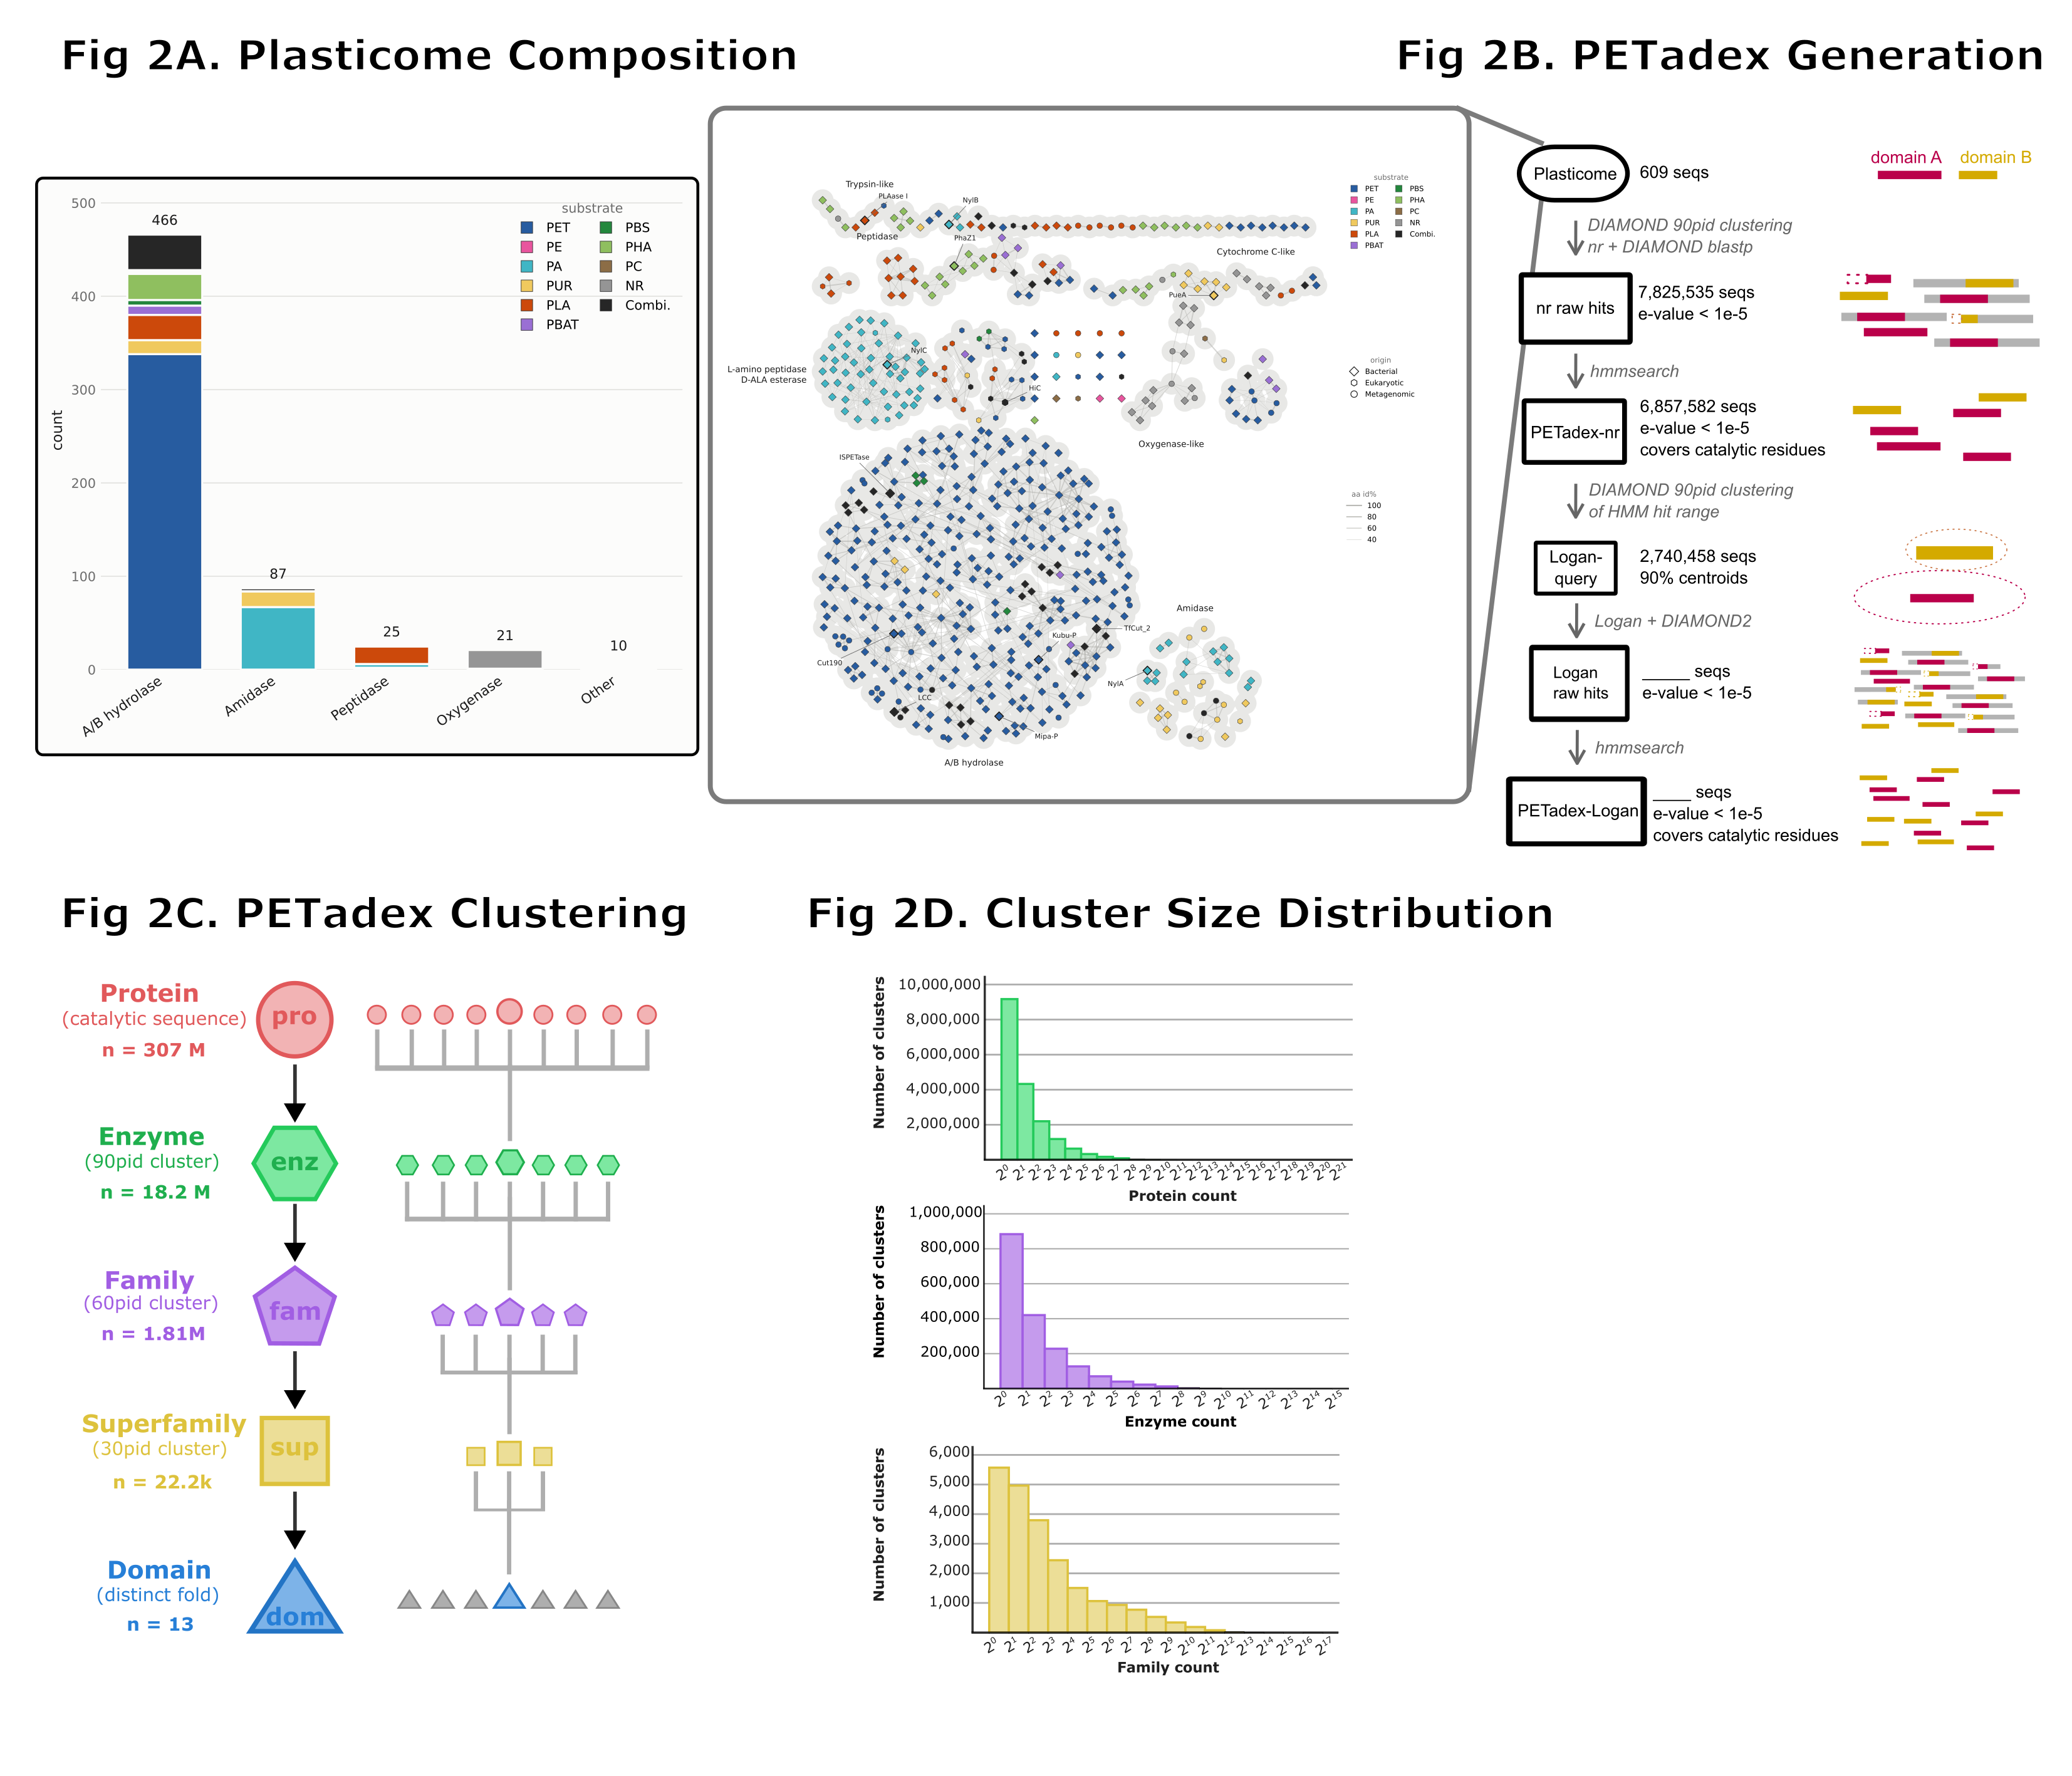
\includegraphics[width=\textwidth]{figures/petadex-manuscript-figure.2_petadex-dataset.png}
\caption{\textbf{The PETadex-260701 dataset.} \textbf{(A)} Composition of the plasticome: the 609-enzyme union of the two PAZy snapshots, its collapse to 411 cluster centroids at 90\% amino acid identity, the 46 graph components those centroids resolve into, and the CATH folds assigned to them, coloured by provenance. \textbf{(B)} Overview of PETadex generation, from the 411 input sequences through the PETadex-nr and PETadex-logan expansions. \textbf{(C)} Hierarchical clustering of catalytic sequences into enzymes (90\% identity), families (60\%), superfamilies (30\%) and distinct folds. \textbf{(D)} Cluster size distributions at the protein, enzyme and family levels.}
\label{fig:dataset}
\end{figure*}

To generate this updated PETadex-260701 dataset, we created a starting search query from combining two versions of the PAZy database, the first from the original PETadex generation (pazy-240826; $n=212$; August 26th, 2024), and a recently updated version (pazy-260701; $n=473$; July 1st, 2026). Sourcing 136 enzymes from pazy-240826, 397 enzymes from pazy-260701 and 76 merged between both, generating a 609 enzyme union set (plasticome). Plasticome was then clustered at 90\% amino acid identity to 411 cluster centroids (Fig.~\ref{fig:dataset}A). Structure- and sequence-based domain assignment of predicted structures resolved the proteins into 15 distinct protein domains, and all-vs-all alignment further groups the centroids into 46 graph components (Fig.~\ref{fig:dataset}A; Methods).
% NOTE (2026-10-01): tool and threshold detail (ESMFold2 ESMC-6B trunk, Foldseek vs CATH S40, InterProScan, the >=30% identity / E < 1e-5 edge criterion) moved to Methods > "Plasticome construction" and "Domain assignment of the plasticome".

\subsection{Homology-based retrieval yields a dataset of 215.7 million putative plastic-degrading enzymes}

To expand the dataset of known PDEs beyond the plasticome set, we first searched these 411 centroids against the NCBI nr database using DIAMOND \todo{cite}, recovering 42,053,081 pairwise alignments, collapsing to 8,850,583 unique sequences. Of these, 7,825,535 pass the e-value filter ($E \le 1\times10^{-5}$), and further removing plasticome self-hits returns a final count of 7,825,107 sequences (Fig.~\ref{fig:dataset}B; Methods).
% NOTE (2026-10-01): DIAMOND version and flags moved to Methods > "Retrieval of homologs from NCBI-nr".

In order to search Logan with only the catalytic domains of these plasticome homologs, we built profile HMMs to characterize the plastic-degrading domain boundaries and catalytic residues. These HMMs were seeded from alignments of plasticome sequences together with their closest nr homologs, where each member of the alignments must contain the residues involved in the catalytic mechanism, annotated from literature \todo{cite}. The 46 graph components were further segmented using these catalytic mechanisms, resolving into 53 seed alignments. Each seed alignment was then expanded over four iterations of a pipeline analogous to JackHMMER \todo{cite}, in which an nr homolog enters the next iteration only if it retains all of the canonical catalytic residues (Methods).
% NOTE (2026-10-01): the iteration procedure (HMMbuild/HMMsearch steps, the 1e-50 and 1e-10 cut-offs, MUSCLE 5.3, the 0.7 occupancy threshold) moved to Methods > "Catalytic-residue-constrained profile HMMs".

% NOTE (2026-10-01): the four counts in this paragraph do not match the counts the vault measured on disk on 2026-09-04 (PETadex/Manuscript/Thomas/Artifact Index.md): 7,562,485 sequences with an HMM hit, 6,764,973 complete catalytic hits, 2,747,171 Logan-query centroids. Left as written here; confirm with T.Q. which run each set comes from before submission.
Searching these component HMMs against the 7,825,107 nr sequences yielded 7,562,397 HMM hits. Of these hits, the HMM range of 6,857,582 contained all of the positions of the catalytic residues (``complete hits''), of which 6,343,582 contained the canonical catalytic residue identities. The ranges annotated as the catalytic domains were then clustered at 90\% identity, resulting in 2,740,458 centroids (Fig.~\ref{fig:dataset}B; Methods). These centroids serve as the input query into Logan.

Expanding on the nr search, we queried these \todo{x} million enzyme homologs across Logan (version \todo{x}) contigs, recovering \todo{x} billion matching sequences (Fig.~\ref{fig:dataset}B). Of these Logan sequences, \todo{x} matched an nr enzyme at 90\% identity, and clustering the remaining \todo{x} at 90\% aaid, yielding \todo{x} million non-redundant enzyme homologs (Fig.~\ref{fig:dataset}C,D). We've dubbed this dataset PETadex-v2, with sub sets dubbed PETadex-plasticome (or simply plasticome), PETadex-nr and PETadex-logan, depending on the origin. \todo{Describe a domain from the search, can be a/B hydrolase, Amydases, etc.}

\subsection{Structural and taxonomic annotation of the PETadex enzyme space}

To explore the PETadex dataset, we annotated its sequences structurally and taxonomically, and linked each sequence to the metadata of the sample it was recovered from.

We first predicted structures for the 22,235 superfamily centroids (30\% amino acid identity) using ESMFold2 \todo{cite ESMFold2} (Methods). These structures resolve both the catalytic domain and the accessory domains flanking it, which may additionally contribute to the catalytic mechanism.

We next assigned each sequence a source organism, from the NCBI taxonomy of its GenBank record (PETadex-nr) or the taxonomic composition of its source run (PETadex-logan). Of \todo{x} PETadex-nr sequences, 1,192,350 (\todo{x}\%) carry an assignment, overwhelmingly bacterial (1,071,209; 89.8\%), followed by Eukaryota (103,380; 8.7\%), Archaea (17,493; 1.5\%) and Viruses (268; $<$0.1\%) \todo{taxonomy panel removed from Fig.~3; cite a Supplementary figure or drop the reference}.

\begin{figure*}[!t]
\centering
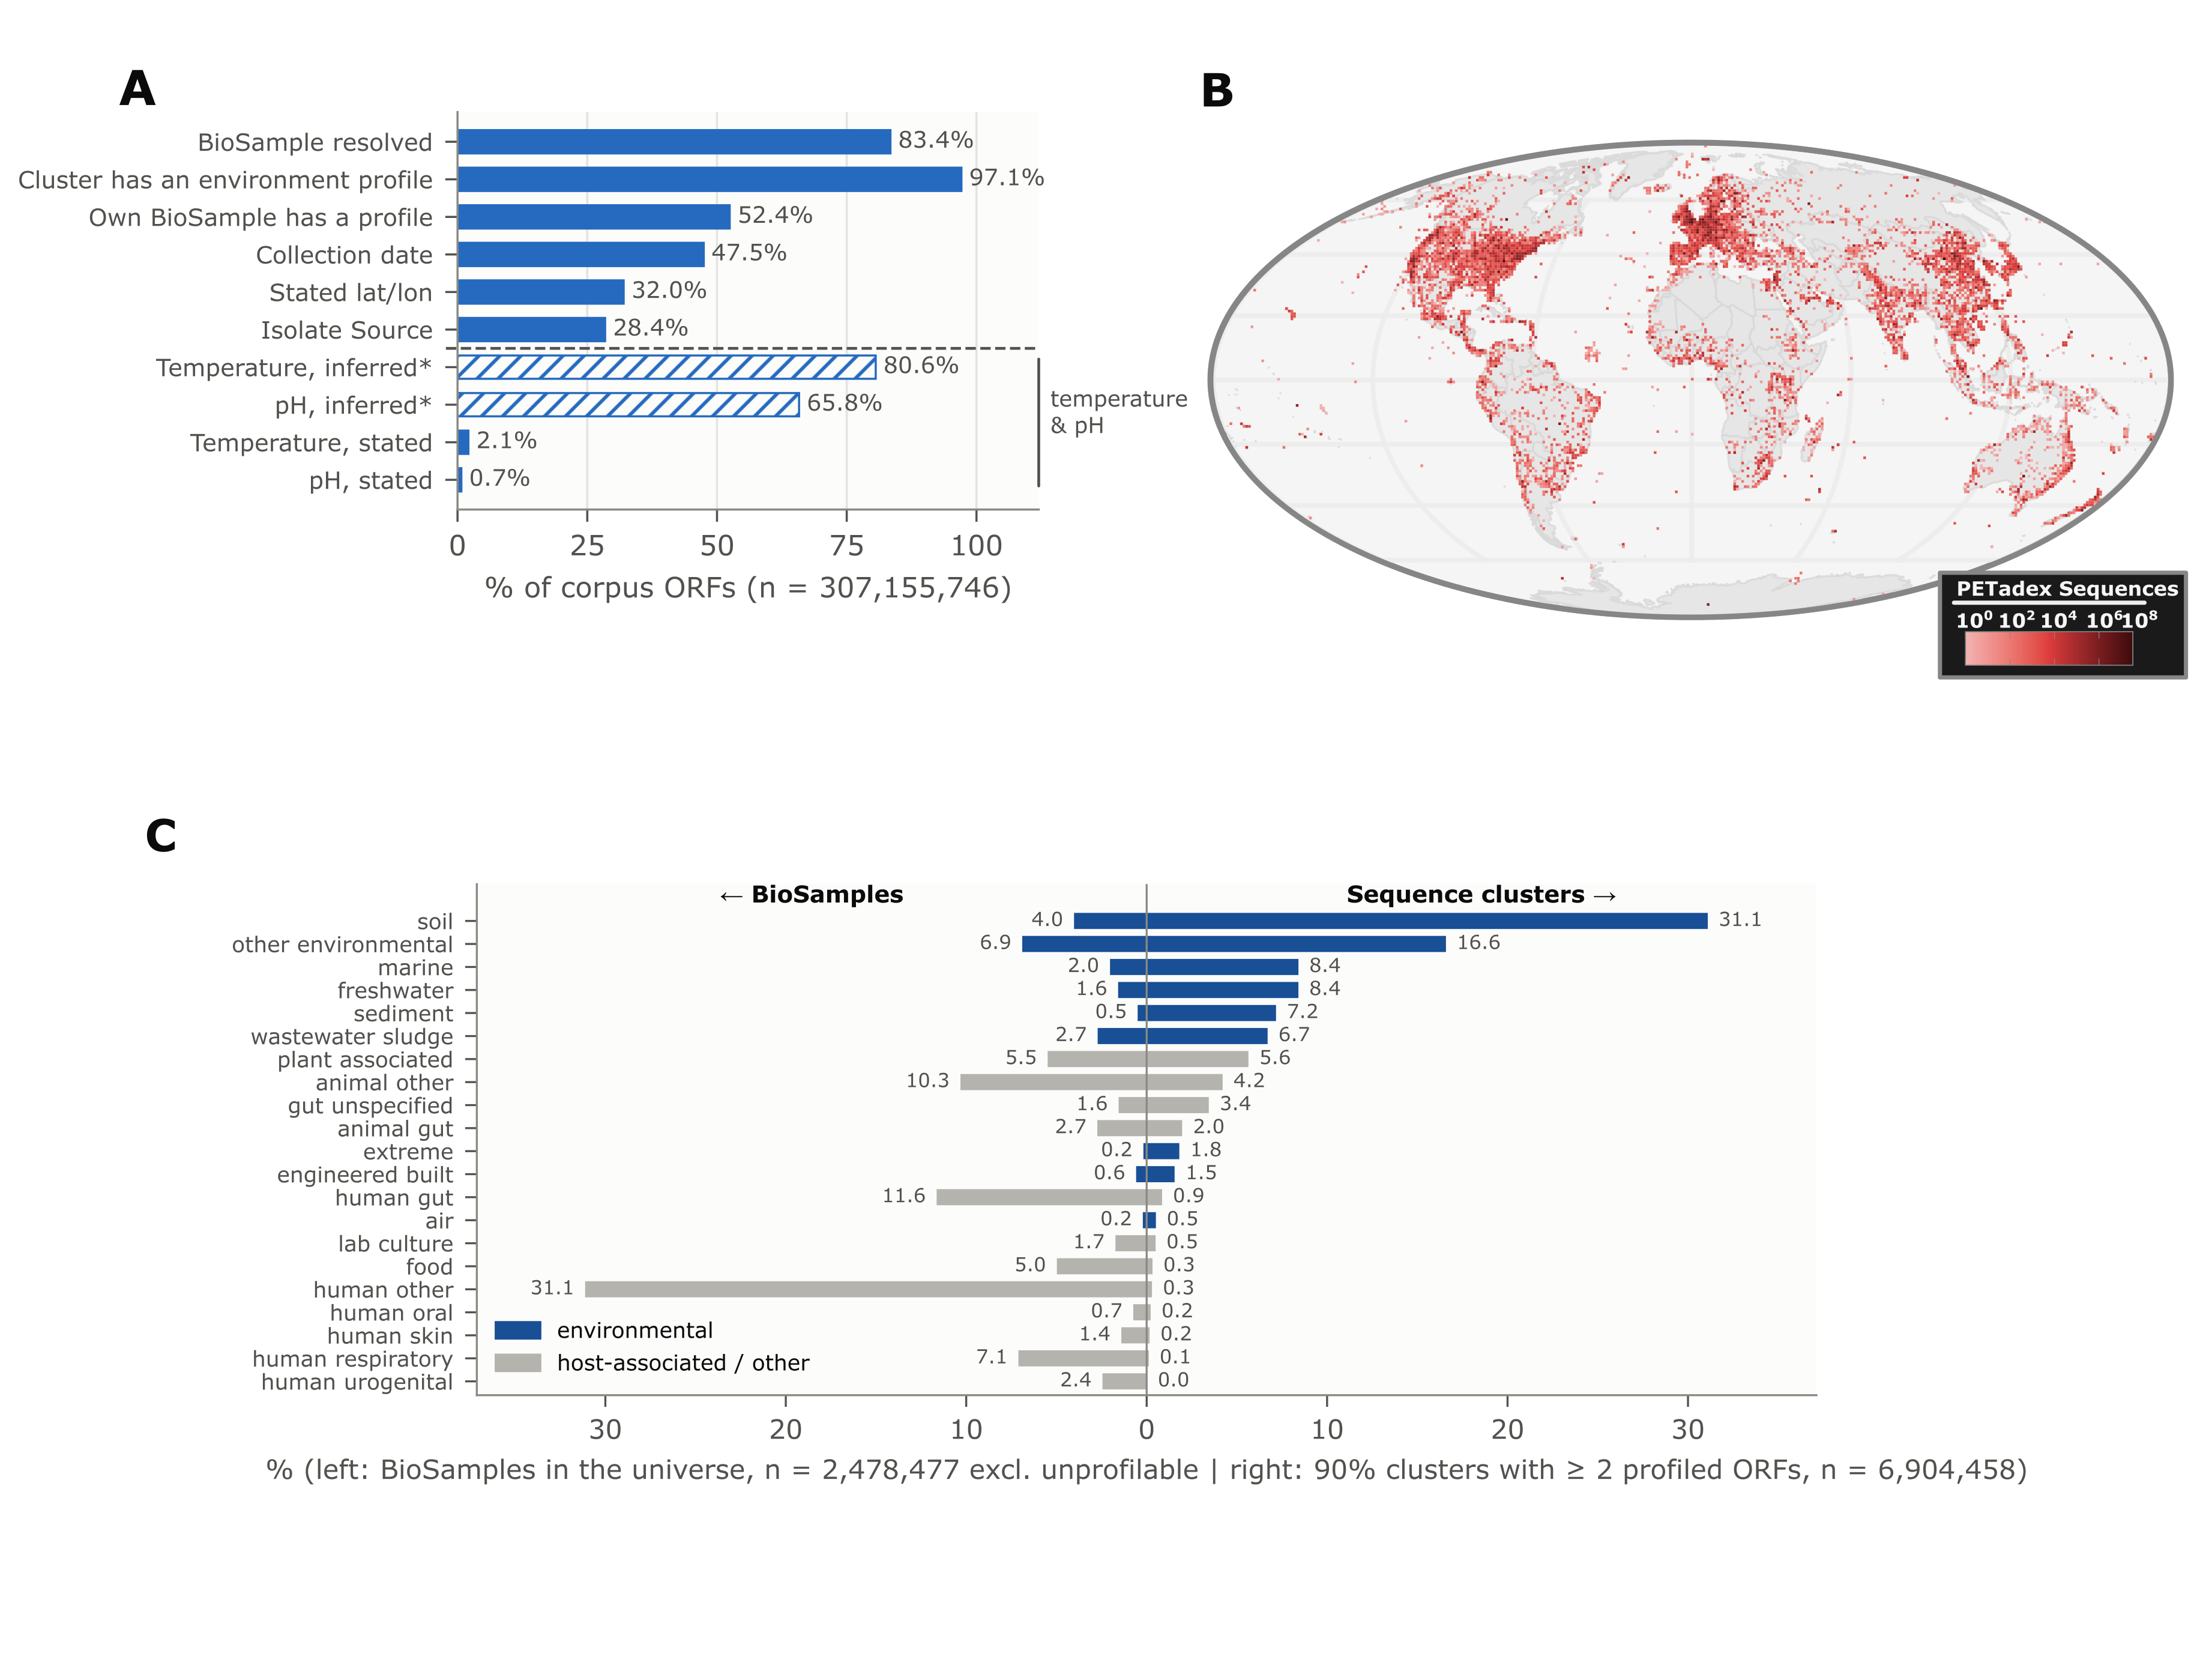
\includegraphics[width=\textwidth]{figures/figure3_metadata.png}
\caption{\textbf{Environmental metadata of the PETadex corpus.} \textbf{(A)} Share of corpus ORFs ($n = 307{,}155{,}746$) with each metadata field. Solid bars, stated in BioSample records; hatched bars (*), inferred from BacDive optima of the taxa in each BioSample. \textbf{(B)} PETadex sequences by stated BioSample coordinates (log scale). \textbf{(C)} Environment categories of profiled BioSamples (left; $n = 2{,}478{,}477$) and of 90\% clusters with $\geq 2$ profiled ORFs (right; $n = 6{,}904{,}458$). Blue, environmental; grey, host-associated or other.}
\label{fig:metadata}
\end{figure*}

\subsection{Sample metadata provides planetary-scale annotation of the PETadex dataset}

Each PETadex-logan sequence is taken from an SRA run, which links to an associated BioSample record, and potentially to an overarching BioProject. These records carry metadata features, such as the location, biome, host, etc., describing the sample, its collection conditions and subsequent sequencing methods. For our dataset of 307,155,746 ORFs, 256,236,322 are linked to BioSamples (83.4\% coverage), drawn from 5,170,787 BioSamples (Fig.~\ref{fig:metadata}A).

Tracking the coverage of the metadata fields for the BioSamples, we can see that the BioSample records are most complete when describing collection date (47.5\%), stated coordinates (32.0\%) and isolation source (28.4\%) (Fig.~\ref{fig:metadata}A). From the geographical coordinates of the samples, we can visualize the truly global span of PETadex putative PDEs, with notable hotspots in North America, Europe and East Asia. It is important to note, however, that the span of these enzymes largely tracks sequencing runs globally, or simply put, these enzymes are found anywhere and everywhere sampling occurs. Other metadata features describing the physical conditions at collection, such as temperature and pH, are rarely documented, with stated temperature available for 2.1\% of ORFs and stated pH for 0.7\%. This reflects the sparse and often unreliable nature of physical condition measurements throughout the SRA.

% NOTE (2026-09-24): 97.1% = 298,257,104 of 307,155,746 ORFs in a 90% cluster with a dominant category, all ORFs counted (f3a_coverage.py, row profile_cluster). The vault's former 82.0% was sum(n_orfs), which counts only BioSample-linked ORFs (251,857,584), over the whole corpus -- do not revert to it. See vault: BioSample Annotation Layer/00 Annotation Layer - Overview.md section 2.
BioSample records are also highly heterogeneous, for instance the isolation source field alone contains 78,439 distinct values. To make these records comparable, and to allow enzyme candidates to be selected for experimental validation by their environment of origin, we classified BioSamples into 21 environment categories based on their stated environment terms, isolation source and host (Methods). Of the 2,744,599 BioSamples carrying at least one usable metadata field, 2,478,477 were assigned a category. Through their BioSample, 52.4\% of the 307 million ORFs receive a category directly. To extend this coverage, we assigned each 90\% sequence cluster the dominant category of its member ORFs and propagated it to members without a category of their own, raising coverage to 97.1\% of ORFs (Fig.~\ref{fig:metadata}A). Counted by BioSample and by cluster, the categories give opposite pictures (Fig.~\ref{fig:metadata}C). Human-associated categories account for 54.3\% of profiled BioSamples, predominantly \textit{human other} (31.1\%) and \textit{human gut} (11.6\%), but only 1.7\% of clusters with at least two profiled ORFs. Environmental categories account for 18.7\% of BioSamples but 82.2\% of clusters, led by soil (31.1\% of clusters) and followed by other environmental sources (16.6\%), marine and freshwater (8.4\% each), sediment (7.2\%) and wastewater sludge (6.7\%). Thus, while sequencing effort in the SRA is dominated by host-associated samples, most of the sequence diversity of PETadex enzymes lies in environmental samples.

% NOTE: inferred temperature still rests on the BacDive cache in which many "optima" are incubator settings (SRA-B3); recompute on the full BacDive pull before submission, or hold temperature out. pH is unaffected.
To improve the sparse metadata annotation for environmental physical conditions of temperature (2.1\%) and pH (0.7\%), we attempt to leverage community species composition for BioSamples. For each run, we first averaged BacDive growth optima of the taxa detected and then weighted by read abundance to obtain an approximation of sample conditons (Methods) \todo{cite BacDive}. This proved effective at raising coverage from 2.1\% to 80.6\% of ORFs for temperature, and from 0.7\% to 65.8\% for pH (Fig.~\ref{fig:metadata}A). These inferred optima describes the organism within a sample, so we validated them against stated measurements for BioSamples where data was available. Abundance-weighted optima correlate with measured pH across 6,473 BioSamples (Pearson $r = 0.34$, against 0.14 without weighting) and with measured temperature across 45,741 BioSamples ($r = 0.16$, against 0.05). These samples are compressed towards neutral pH and mesophilic temperatures, and therefore do not improve on a constant in absolute error. We therefore propose that inferred optima can be applied as a means of ranking and filtering samples, but is not reliable as an estimate of \textit{in situ} conditions, and should thus be treated as distinct from stated values. 


Together these annotations support homology-based characterization of afore uncharacterized enzymes, and allow candidates to be filtered on catalytic integrity, fold and habitat prior to testing.

%% >>>>>>>>>> AI-GENERATED DRAFT (Claude, 2026-09-30) -- REWRITE BEFORE SUBMISSION >>>>>>>>>>
%% Super (Obsidian, Plans and Reflections, 2026-09-30). Treat it as a
%% placeholder to rewrite in your own words. Numbers marked \todo{} are unverified.
%% The plan's caveat: every number and screenshot must come from the Next.js/Vercel
%% rebuild, not the current Gatsby site.
%%
%% Original (human-written) text of this subsection, kept for reference:
%%   This homology-based characterization pipeline is implemented through a DIAMOND
%%   sequence search interface available freely at petadex.net. This sequence search runs
%%   20 shards in parallel to achieve an average search time of ~47 seconds over the
%%   database of ~215.7 million enzymes.
%% NOTE: the plan gives 32 shards / ~44 s over ~307M ORFs, which conflicts with the above
%% (20 shards / ~47 s / 215.7M). Re-benchmark on the rebuild and use one set of numbers.
\subsection{PETadex makes every annotation layer queryable}

% AI-GENERATED -- paragraph 1: data model
To make the dataset and its annotations usable for enzyme discovery, we built PETadex as an openly accessible web resource (\url{https://petadex.net}) in which every annotation layer described above can be queried and cross-referenced. The database is organized around six linked entity types: sequences (307,155,746 ORFs); their cluster centroids at 90\%, 60\% and 30\% amino acid identity; the 609 plasticome reference enzymes; the BioSamples the sequences were recovered from; the plastic substrates (polymers) that the reference enzymes act on; and kinetic measurements linking reference enzymes to substrates. Because these entities are linked, a user can traverse from any putative enzyme to its cluster centroid, from the centroid to its nearest characterized plasticome enzyme and that enzyme's known substrates and kinetics, and from the sequence to the environmental metadata of the sample it came from.

% AI-GENERATED -- paragraph 2: search
The main entry point is sequence search. Query proteins are searched against the full PETadex corpus with DIAMOND \todo{cite DIAMOND}, which we split into \todo{32} shards searched in parallel, giving an end-to-end latency of $\sim$\todo{44}\,s per query (Methods) \todo{add latency vs corpus size and/or query length, ideally as a Supplementary figure}. Each search is stored with a persistent URL, so a result set can be shared or cited and later retrieved without being recomputed, which makes candidate selection from PETadex reproducible. Each hit links to a sequence page that reports its cluster memberships, closest plasticome enzyme, source organism and BioSample metadata.

% AI-GENERATED -- paragraph 3: browse layers
Alongside search, PETadex provides four browsable layers. The ESM Atlas is an interactive embedding map of the 64,730 \todo{60\%?} family centroids, where users can locate plasticome enzymes and explore uncharacterized neighbourhoods of sequence space in ESM-2 embedding space \todo{cite ESM-2}. Predicted ESMFold2 structures of the 22,235 superfamily centroids can be viewed in the browser from each centroid page. The Enzyme Activity layer collects 464 kinetic records for plasticome enzymes against a library of 20 polymer substrates, curated from the literature (Methods). The BioSample layer exposes the environmental metadata of each sample, including the 21 environment categories and the stated and inferred temperature and pH described above (inferred values cover 80.6\% of ORFs for temperature and 65.8\% for pH), with inferred values labelled separately from stated ones.

% AI-GENERATED -- paragraph 4: open access
All PETadex data are openly available. Sequences, cluster assignments, annotations and metadata can be downloaded in bulk from public Amazon S3 buckets \todo{bucket names/URLs}, and the PlasticESM model and its training set are released on Hugging Face \todo{URL}. Data are released under \todo{licence, e.g.\ CC BY 4.0}, and the source code for the website and search infrastructure is available on GitHub (Code availability).

% Website figure removed (2026-09-30): Fig. 4 is reserved for the superfamily case study
% (IsPETase-LCC). If the website gets a figure later (entity-graph schematic + search /
% sequence page / Atlas screenshots from the rebuild), it goes in the Supplementary.
%% <<<<<<<<<< END AI-GENERATED DRAFT (Website subsection) <<<<<<<<<<

%% >>>>>>>>>> AI-GENERATED DRAFT (Claude, 2026-09-30) -- REWRITE BEFORE SUBMISSION >>>>>>>>>>
%% Superfamily case study. Written from the Obsidian vault, PETadex/Projects/Superfamily
%% Case Study (IsPETase-LCC): Overview.md, Review 2026-09-28 - Response.md (verified
%% numbers), T9SS-CTD Lineage 2026-09-30.md, Composite v1/v2 caption notes.
%%
%% IMPORTANT -- WHICH COMPOSITE THIS IS. The committed PNG
%% (figure_4_superfamily-case-study_composite.png) is COMPOSITE v1: panel A carries the
%% sample-type and environment rings, panel B is the 563-tip linear tree, and panel C is
%% ORF-weighted. The vault marks v1 superseded by v2, in which A gains the Logan-fraction /
%% family-size / enrichment rings, B becomes an architecture strip over all 41,871 members,
%% and C moves to 90% cluster level (the Logan-vs-nr gap falls from 17 to 6 points). The
%% caption below therefore describes v1, because that is the image. Swap in the v2 PNG and
%% the v2 caption (in the vault) before submission, or the caption will not match the figure.
%%
%% ALSO OPEN in the vault: the thesis of this figure is not yet agreed with Artem, and the
%% choice in panel C between leading with the Logan-vs-nr divergence or with "62% of 90%
%% clusters are Logan-only" is undecided. The prose below takes the review's proposed
%% thesis (characterized enzymes sample a narrow, nr-centric corner of the superfamily).
\subsection{A single superfamily shows that characterized enzymes sample a narrow corner of the sequence space}

% AI-GENERATED -- paragraph 1: the superfamily as a worked example
To show how these annotation layers combine in practice, we examined one 30\% identity superfamily in detail: superfamily 6, the $\alpha/\beta$-hydrolase superfamily (CATH 3.40.50.1820) that contains both IsPETase and LCC, along with the two further reference enzymes Cut190 and TfCut2 \todo{cite Cut190, TfCut2}. It contains 41,871 ORFs, 32,230 of them from Logan and 9,565 from NCBI-nr, resolving into 407 families at 60\% identity and 5,532 clusters at 90\% identity. Of these 90\% clusters, 62\% are recovered only from Logan, and 129 of the 407 families contain Logan sequences alone. Characterized plasticome enzymes fall in just 40 of the 407 families, so most of the superfamily has no characterized representative at all.

% AI-GENERATED -- paragraph 2: phylogeny and environment
We inferred a maximum-likelihood phylogeny of 563 representatives of the superfamily: the 388 family centroids, 161 characterized plasticome enzymes, the four reference enzymes and two centroids from neighbouring superfamilies (Fig.~\ref{fig:superfamily}A; Methods). The neighbouring superfamily centroids nest inside superfamily 6 rather than outside it, and no candidate outgroup we tested fell outside the superfamily, so the tree is midpoint-rooted and the 30\% identity boundary is an operational unit rather than a clade. The deep backbone is weakly supported (15\% of nodes below 70\% UFBoot) and we do not interpret deep branching. The superfamily is nonetheless environmentally structured rather than cosmopolitan: testing each family for enrichment of an environment category against the rest of the superfamily, counting distinct BioProjects so that a single large study cannot drive an enrichment, 82 of 130 testable families are significantly enriched for one category (one-sided Fisher, Benjamini--Hochberg $q < 0.05$), most often soil (26 families), aquatic (17) or engineered environments (15) \todo{this enrichment analysis is panel A of composite v2, not of the v1 figure committed here; either swap the figure or cite a Supplementary panel}.

% AI-GENERATED -- paragraph 3: architecture and the T9SS lineage
Domain architecture across the superfamily is highly uniform: the $\alpha/\beta$-hydrolase core is present in 41,815 of the 41,871 members (99.9\%) and occurs alone in 91.8\% of them, and the canonical Ser-Asp-His catalytic triad is conserved in 548 of the 555 representatives present in the corpus (Fig.~\ref{fig:superfamily}B). The remaining 7.3\% of members, drawn from 47 families, carry an accessory domain \todo{cite Pfam}. The most frequent is the type-IX secretion system C-terminal sorting domain (T9SS-CTD, PF18962; 1,662 members in 24 families, 84\% of them from Logan), followed by a Ricin-B lectin (729 members) and the carbohydrate-binding module CBM2 (324). The T9SS-CTD marks a Bacteroidota radiation on the opposite side of the tree from all four reference enzymes, and is more deeply phylogenetically conserved than any environmental or sample-type trait we measured on this superfamily (consenTRAIT $\tau_D$ 1.45-fold the permuted null on the family tree, $p = 0.002$) \todo{cite consenTRAIT}, though less so than host taxonomy. Only two characterized enzymes, PET30 and PET27, sit within it \todo{cite PET30, PET27}. Its largest family (2,287 ORFs, 97.6\% from Logan, drawn from 438 BioProjects and enriched in engineered environments, mostly wastewater sludge, with freshwater samples next most common) sits at a median 46.7\% identity to any characterized enzyme, making the secretion-tagged lineage a concrete example of a candidate group that is invisible to a search of characterized sequences alone.

% AI-GENERATED -- paragraph 4: novelty
Finally, we measured how far this diversity sits from what has been characterized (Fig.~\ref{fig:superfamily}C,D). Logan members lie a median 61.8\% identity from their nearest characterized enzyme, against 78.9\% for nr members, with 32\% and 11\% respectively below 50\% identity. This comparison is ORF-weighted, and because near-identical nr sequences pile up in a few large clusters next to characterized enzymes it overstates the difference: at 90\% cluster level the medians are 56.5\% (Logan-only) and 62.3\% (nr-only), a gap of 6 points rather than 17, still significant (Mann--Whitney $p = 1.5\times10^{-7}$) but modest \todo{decide which unit the figure and text report; composite v2 shows the cluster-level version}. Some of this difference is expected by construction, since characterized enzymes come from cultured organisms deposited in nr. The reference enzymes themselves have strikingly few close relatives: only 41 (LCC) to 233 (Cut190) of the 41,871 members are $\geq$90\% identical to a reference, and an exhaustive search of all nr and PAZy ORFs together with every 60\% family centroid found no closer homolog anywhere else in PETadex. Most of the superfamily is 30--50\% identical to all four references. The characterized enzymes that anchor this field therefore sample a narrow corner of the sequence space their own superfamily occupies.

% AI-GENERATED -- Fig. 4. NOTE: this PNG is composite v1 (8800x8000 RGBA, ~5.8 MB); the
% caption matches it. Downsample to 600 DPI before committing the PDF (see CLAUDE.md).
\begin{figure*}[!t]
\centering
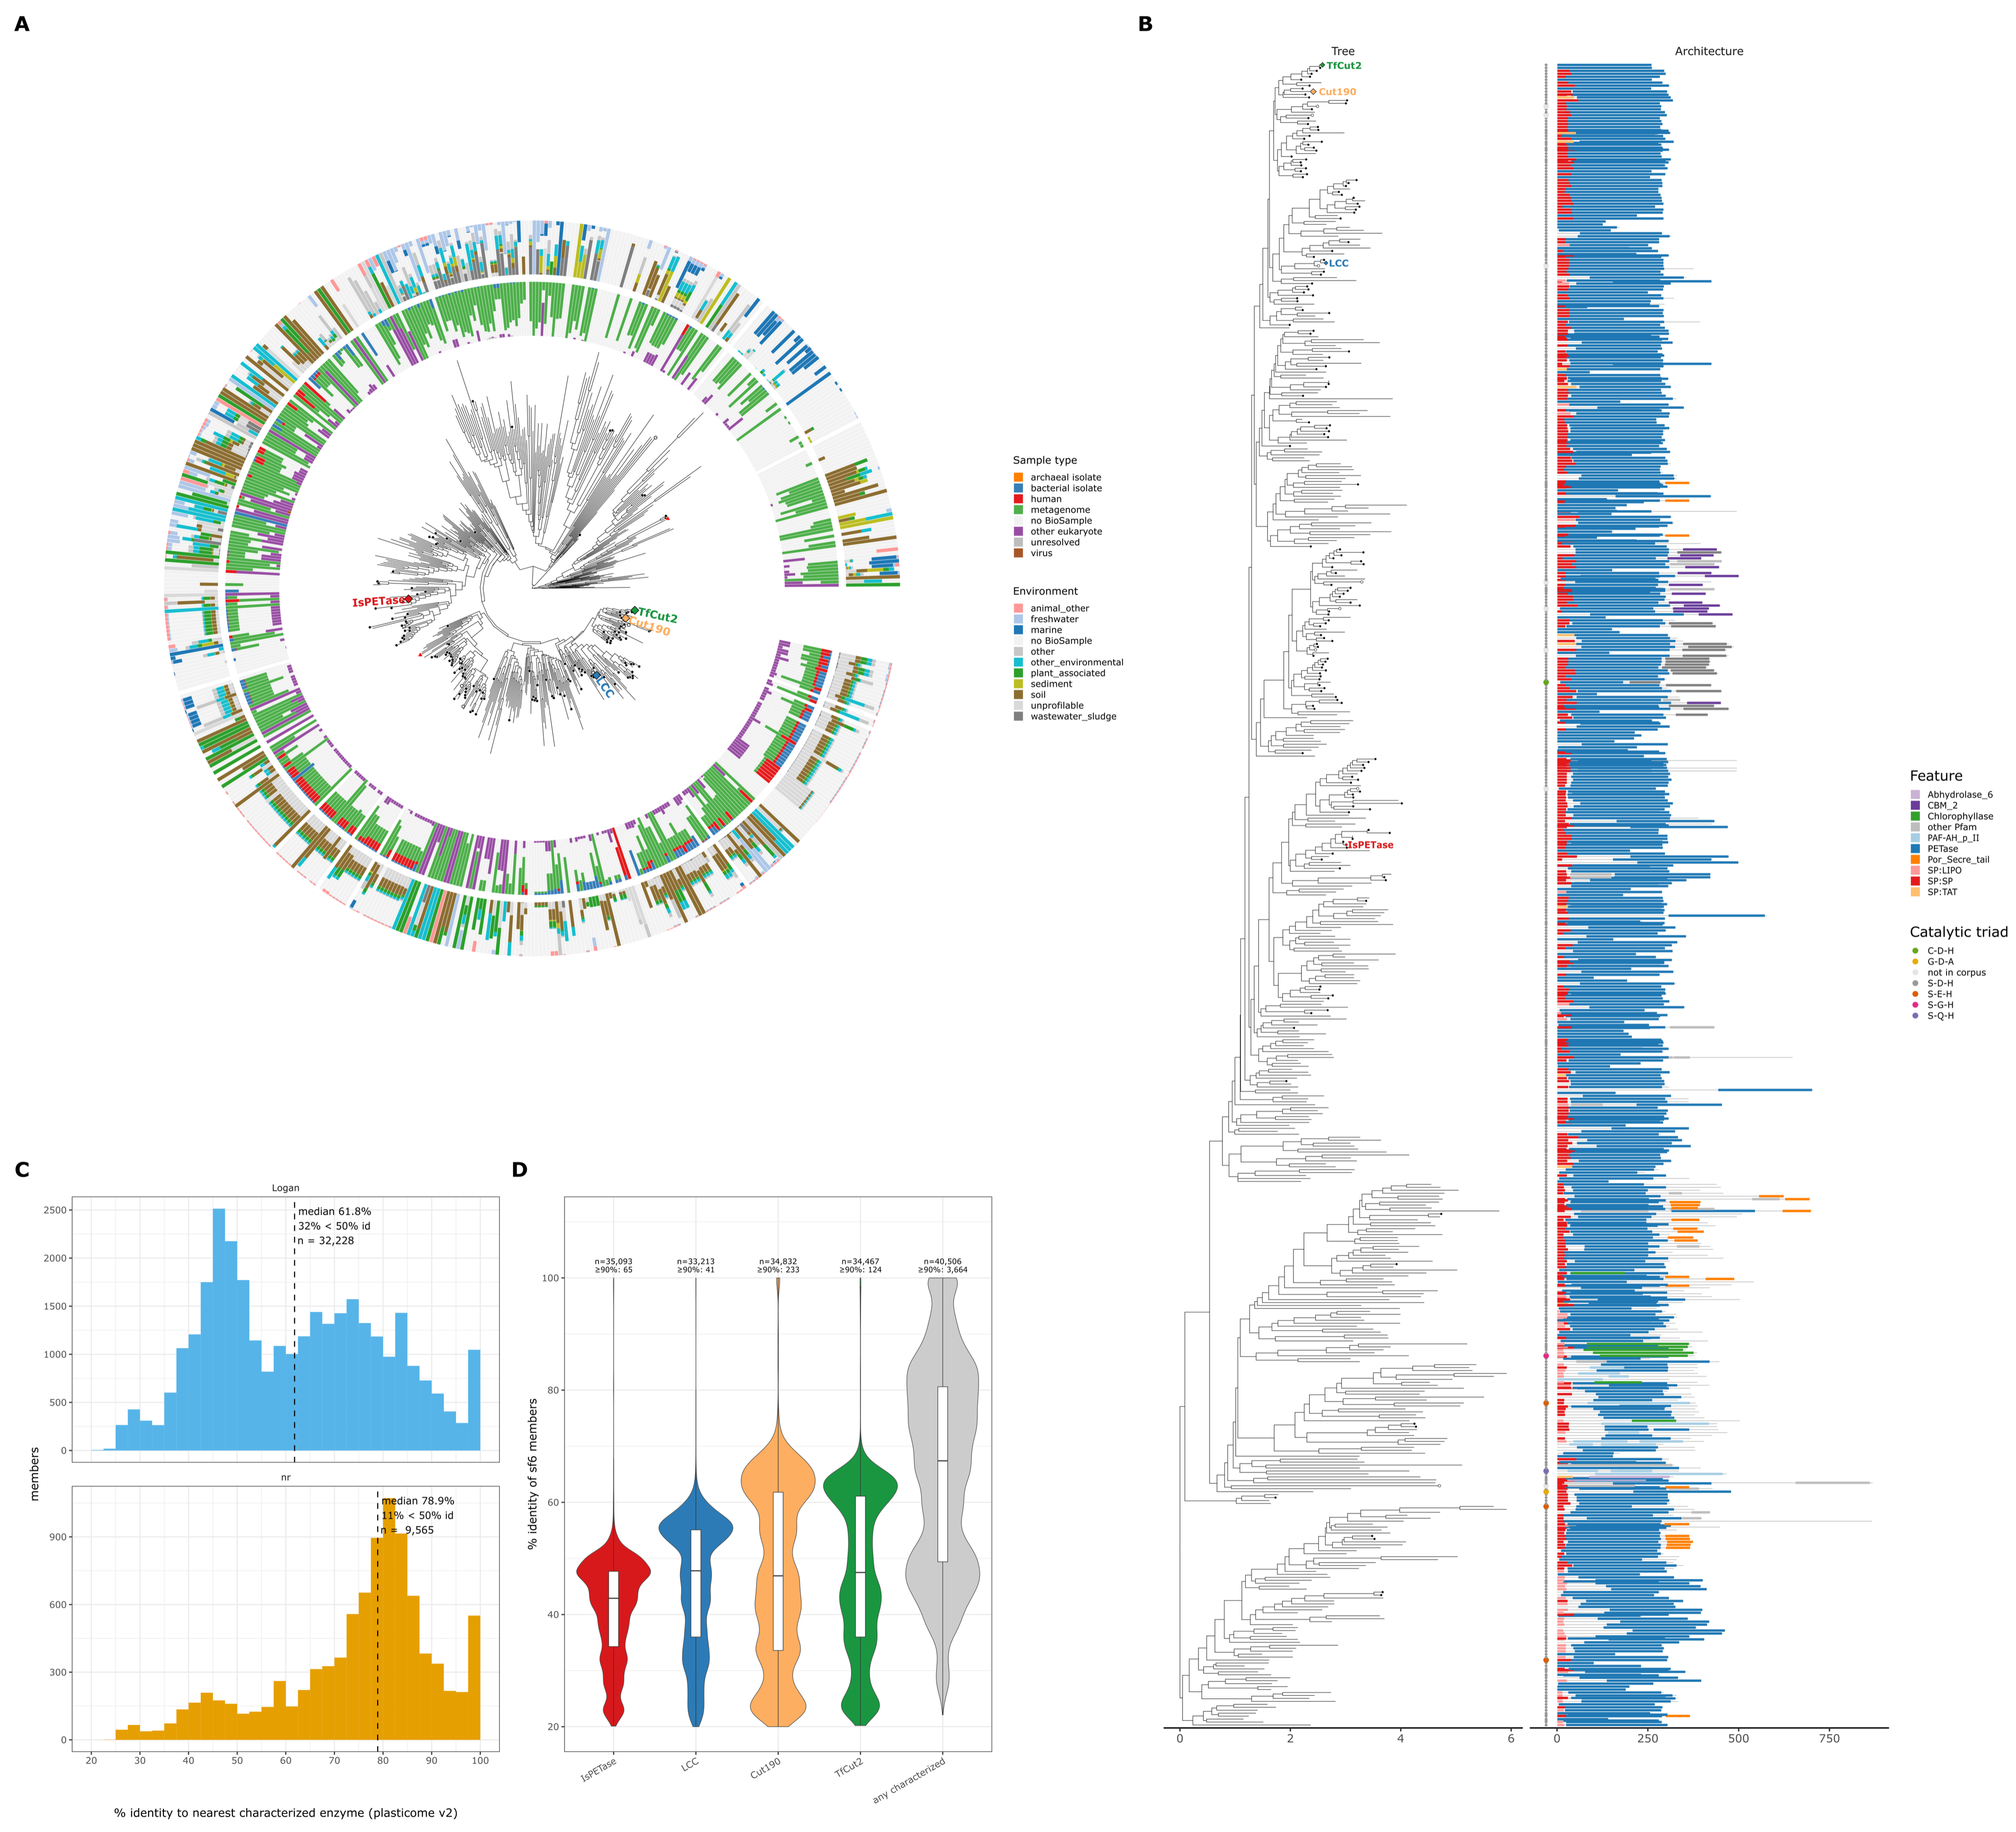
\includegraphics[width=\textwidth]{figures/figure_4_superfamily-case-study_composite.png}
\caption{\textbf{Characterized PET hydrolases sample a narrow corner of the IsPETase/LCC superfamily, most of whose diversity is recovered only from Logan.} PETadex superfamily 6 (30\% identity cluster) contains 41,871 ORFs, 77\% of them from Logan assemblies of SRA runs, in 407 families at 60\% identity. The superfamily is an operational unit, not a clade: neighbouring superfamilies nest within it. \textbf{(A)} Maximum-likelihood phylogeny (IQ-TREE, WAG+F+I+R10, midpoint-rooted) of 563 representatives: 388 family centroids (60\% identity), 161 characterized plasticome enzymes (filled dots), 8 characterized sequences absent from PETadex (open dots), the four reference enzymes IsPETase, LCC, Cut190 and TfCut2 (diamonds), and 2 neighbouring-superfamily centroids (red triangles). The deep backbone is weakly supported and is not interpreted. Rings, inner to outer: sample type and environment category of each family's BioSamples. \textbf{(B)} The same tree drawn linearly, with the domain architecture of each representative: Pfam domains, SignalP~6.0 signal peptides, and the catalytic triad (dots; Ser-Asp-His in 548 of the 555 representatives present in the corpus). \textbf{(C)} Identity of each member to its nearest characterized enzyme (plasticome v2). Logan members: median 61.8\%, 32\% below 50\% ($n = 32{,}228$). nr members: median 78.9\%, 11\% below 50\% ($n = 9{,}565$). nr is enriched near characterized enzymes by construction. \textbf{(D)} Identity of every member to each reference enzyme, and to any characterized enzyme. Only 41 (LCC) to 233 (Cut190) members are $\geq$90\% identical to a reference.}
\label{fig:superfamily}
\end{figure*}
%% <<<<<<<<<< END AI-GENERATED DRAFT (Superfamily case study) <<<<<<<<<<

%% ============================================================
%% Discussion
%% ============================================================
\section{Discussion}

%% >>>>>>>>>> AI-GENERATED DRAFT (Claude, 2026-09-30) -- REWRITE BEFORE SUBMISSION >>>>>>>>>>
%% Website/resource paragraph from the website-section plan. Positioning, limitations,
%% sustainability and future layers. Reviewers ask about sustainability for resource
%% papers, so keep that part in some form even if the rest is cut.
PETadex complements, rather than replaces, curated resources of plastic-degrading enzymes. PAZy \todo{cite PAZy} and PlasticDB \todo{cite PlasticDB} catalogue experimentally characterized enzymes, and PMBD \todo{cite PMBD} collects plastic-degrading microorganisms and genes from the literature. PETadex is several orders of magnitude larger, is derived mainly from metagenomes, and pairs each sequence with the environmental context of its source sample, while linking back to characterized enzymes through the plasticome. This scale has limits. Apart from the plasticome, PETadex entries are putative enzymes that have not been validated experimentally, and the website labels them as such \todo{confirm the rebuild shows this on every non-plasticome page}. Environmental metadata are recorded per sample, not per ORF, so they describe where a sequence was found rather than the conditions its enzyme is adapted to. To keep the resource maintainable, PETadex is released in numbered versions (the present release is PETadex-260701), and it runs on serverless infrastructure whose costs scale with use rather than with uptime \todo{give the maintenance plan and funding horizon, plus approximate monthly cost}. Future releases will add new annotation layers, including novel domain and TED structural-domain annotations \todo{cite TED}, feed wet-lab assay results for PETadex candidates back into the Enzyme Activity layer, and accept community submissions of characterized enzymes.
%% <<<<<<<<<< END AI-GENERATED DRAFT (Discussion: resource paragraph) <<<<<<<<<<

%% ============================================================
%% Methods
%% ============================================================
\section{Methods}

%% >>>>>>>>>> AI-GENERATED DRAFT (Claude, 2026-10-01) -- REWRITE BEFORE SUBMISSION >>>>>>>>>>
%% Dataset-generation and annotation Methods, ordered by pipeline rather than by Results
%% heading. Two sources: (1) methods detail lifted out of Results on 2026-10-01 (the HMM
%% iteration procedure, the 0.7 occupancy threshold, the MUSCLE/DIAMOND flags, the plasticome
%% structure/CATH tooling; see the NOTE comments in Results), and (2) the Obsidian vault:
%%   Plasticome construction ...... PETadex/Projects/Logan Work/Runs/Plasticome pipeline end to end.md
%%                                  PETadex/Projects/Logan Work/Documentation/Plasticome v2 Build Overview.md
%%   Domain assignment ............ PETadex/Projects/Plasticome CATH Assignment/00 Project Overview.md
%%   Structure prediction ......... PETadex/Projects/Narval Folding/ESMFold2 Plasticome Folding.md
%%   NCBI-nr retrieval, HMMs ...... PETadex/Manuscript/Thomas/ (Overview, HMM_Documentation, Seed MSAs and
%%                                  Reference Structure Annotations, PETadex-HMM Creation, Artifact Index)
%%   Logan search, clustering ..... PETadex/Projects/Logan Work/Documentation/petadex.v260701_generation-thomas.md
%%                                  (a PLAN, written before the run -- hence the \todo{}s)
%%   BioSample metadata ........... PETadex/Manuscript/Metadata Section/Metadata Section - Writing Notes.md
%%                                  PETadex/Projects/Metadata/Metadata Profiles Experiment/01 Profiles - Method and Decisions.md
%%   Inferred temperature and pH .. PETadex/Projects/Metadata/SRA Metadata Acquisition/pH Metadata/04 How pH_env Is Computed.md
%% Anything the vault does not record is a \todo{}; nothing here was filled in by guessing.
%%
%% CORPUS CAVEAT (vault: Manuscript/Figures Generation/00 Figure Data Extraction - Server Plan.md,
%% section 0). The plasticome, nr and HMM subsections describe PETadex-260701 (v2). The Logan
%% ORF count (307,155,746), the 22,235 superfamily centroids and every metadata number in
%% Results/Fig. 3 are from the v1 corpus, because the v2 Logan search and the metadata rebuild
%% were not finished when those notes were written. The Logan and metadata subsections below
%% describe the method; their counts must be regenerated on v2.

\subsection{Plasticome construction}

% AI-GENERATED -- paragraph 1: PAZy snapshots, curation, union
The plasticome is the union of two snapshots of the PAZy database \todo{cite PAZy}: pazy-240826 (26 August 2024; $n=212$), the seed set of the original PETadex build \todo{cite PETadex v1}, and pazy-260701 (1 July 2026) \todo{confirm the pull date; the vault's reconciliation notes give 2026-06-30 for the same snapshot}. The 495 records in the 2026 snapshot were curated manually against their source publications: 26 records without experimentally reported activity were removed and 4 sequences were added (one reported in the literature but absent from PAZy, one replacing an inactive PAZy record, and two that PAZy aggregates under a single identifier), leaving 473 enzymes. Each enzyme was additionally annotated for whether its activity was demonstrated directly (purified enzyme) or indirectly \todo{state how indirect-evidence enzymes were handled, and give the curation table as a Supplementary Table}. The two snapshots were joined on accession, ignoring accession version, giving a union of 609 enzymes: 397 from pazy-260701 only, 136 from pazy-240826 only and 76 present in both. Sequences were retrieved by accession from NCBI Protein, falling back in order to UniProt, RCSB PDB, coding-sequence translations in NCBI Nucleotide, MGnify and UniParc; a manually curated sequence was used for enzymes with no resolvable accession \todo{Supplementary Table: accession, source snapshot and sequence provenance of all 609 enzymes}.

% AI-GENERATED -- paragraph 2: 90% clustering
The 609 sequences were clustered at 90\% amino acid identity with USEARCH v11.0.667 \todo{cite USEARCH} in a reference-seeded scheme. Thirteen well-characterized enzymes \todo{list the 13 curated seeds in a Supplementary Table} were fixed as cluster centroids, the remaining sequences were first recruited to these centroids (\texttt{usearch\_global -id 0.9 -top\_hit\_only}), and those left unassigned were clustered \textit{de novo} with centroids chosen by decreasing length (\texttt{cluster\_fast -id 0.9 -sort length}). This produced 411 clusters (13 reference-seeded and 398 \textit{de novo}; 272 singletons). The 411 centroids are the query set for the NCBI-nr search. Separately, collapsing the plasticome at 100\% identity gives 493 non-redundant proteins, which were used to seed the profile HMMs.

% AI-GENERATED -- paragraph 3: component graph
Graph components follow the definition used in Logan \todo{cite Logan}: connected components of the all-vs-all amino acid similarity graph. The 411 centroids were aligned all-vs-all with USEARCH v11.0.667 (\texttt{-allpairs\_local -acceptall}, run over both query--target orientations), and the highest-scoring alignment by bit score was kept for each pair. Thresholds were applied after the search, not as search parameters, because identity and e-value thresholds given to the aligner prune candidate pairs before alignment and under-connect the graph. Pairs with $\ge$30\% amino acid identity and $E < 1\times10^{-5}$ (22,203 of 30,588 aligned pairs; e-values as reported for the 144,560-residue database) were taken as edges, and single-linkage connected components of this graph define the 46 components (25 containing a single centroid; the largest containing 232).

\subsection{Domain assignment of the plasticome}

% AI-GENERATED -- CATH by two routes
Structures of all 609 plasticome enzymes were predicted with ESMFold2 (see Structure prediction). CATH homologous superfamilies were assigned by two independent routes and compared. In the structure-based route, predicted structures were segmented into domains with Merizo \todo{cite Merizo; version} and each domain was searched with Foldseek \todo{cite Foldseek; version} against the CATH S40 non-redundant domain set (CATH v4.3.0, with results confirmed against v4.4.0) \todo{cite CATH}, accepting hits with TM-score $\ge 0.5$ and $E \le 1\times10^{-5}$; domains without a hit were searched against TED50 \todo{cite TED} under the same thresholds. In the sequence-based route, sequences were scanned with the CATH-Gene3D HMM library (v21.0.0) and overlapping hits were resolved with cath-resolve-hits \todo{cite Gene3D, cath-resolve-hits}. Assignments were compared at the four-level CATH code, and the two routes agreed for all 643 domains matched by both. A CATH superfamily was assigned to 400 of the 411 centroids. The remaining 11 form a single component of rubber oxygenases (Pfam PF09995), a domain with no CATH superfamily in either release, and were annotated from Pfam (release 38.2) \todo{cite Pfam}. \todo{Results says ``InterProScan'' and ``15 distinct protein domains''. The vault records Gene3D + cath-resolve-hits for the sequence route, and the count of 15 comes from the catalytic annotation table. State where InterProScan was used and how the 15 were counted.}

\subsection{Retrieval of homologs from NCBI-nr}

% AI-GENERATED -- DIAMOND parameters, filters, self-hit removal
The NCBI nr protein database \todo{download date / release of nr} was exported to FASTA with \texttt{blastdbcmd} (BLAST+ 2.17.0) and formatted as a DIAMOND database (DIAMOND v2.2.4.184; 1,101,054,423 sequences, 417,051,418,494 residues) \todo{cite DIAMOND, BLAST+}. The 411 plasticome centroids were searched against it with \texttt{diamond blastp -{}-very-sensitive -k0}, the latter removing the limit on target sequences reported per query. An nr sequence hit by more than one query was assigned to its lowest-e-value query, and inherits that query's graph component. Sequences with $E \le 1\times10^{-5}$ were retained. Retained sequences matching a plasticome protein by accession or by exact amino acid sequence were removed from the nr set (428), so that PETadex-plasticome and PETadex-nr are mutually non-redundant at 100\% identity.

\subsection{Catalytic-residue-constrained profile HMMs}

% AI-GENERATED -- paragraph 1: catalytic residue annotation
For each of the 15 protein domains in the plasticome, the residues required for catalysis were annotated from the mechanistic literature and anchored to a reference sequence with a solved or predicted structure \todo{cite the mechanism papers; give the per-domain catalytic residues, reference structures and sources as a Supplementary Table -- the annotation currently exists only as a Google Sheet}. Where cofactors make no single residue strictly essential, the conserved metal- or cofactor-ligating residues were used instead. Components whose members could not be aligned to their domain's reference with every catalytic residue in the expected column were given a component-specific reference, annotated by structural alignment to the domain reference in PyMOL.

% AI-GENERATED -- paragraph 2: seed MSAs
Seed alignments were built per component from the plasticome sequences and their close nr homologs. Signal peptides were predicted and removed with SignalP~6.0 \todo{cite SignalP}. For each component, nr homologs with $E \le 1\times10^{-50}$ to a plasticome query were clustered with DIAMOND \texttt{linclust}, at an identity threshold chosen by component size (30\% for components of more than 50,000 homologs, 50\% for more than 10,000, 70\% for more than 100 and 90\% otherwise) so that each component was reduced to roughly 100--1,000 sequences. Sequences were aligned with MUSCLE~5.3 (Super5 algorithm) \todo{cite MUSCLE}, and any sequence lacking the annotated residue at a catalytic column was removed. Accessory domains and unaligned N- and C-terminal regions were then trimmed manually, and the trimmed alignments were realigned with the MUSCLE PPP algorithm (Super5 for the cytochrome P450 component, for which PPP did not complete in reasonable time). Components whose members could not all be aligned on one set of catalytic columns were split into sub-components, each with its own reference, giving 57 alignments from the 46 components. Four of these, consisting of fragments or of enzymes with no known mechanism, were discarded, leaving 53 seed alignments.

% AI-GENERATED -- paragraph 3: the iterative build (procedure moved from Results)
Profile HMMs were built from the seed alignments with HMMER~3.4 \todo{cite HMMER} by an iterative procedure analogous to JackHMMER \todo{cite JackHMMER}, with the added constraint that catalytic residues are conserved. In each iteration, (i) a profile was built from the current alignment with \texttt{hmmbuild}; (ii) the reference sequence was aligned to the profile with \texttt{hmmalign}, mapping its catalytic positions onto match states; (iii) the profile was searched with \texttt{hmmsearch} against the nr homologs of its component with a DIAMOND $E < 1\times10^{-10}$, using the size of nr as the search space (\texttt{-Z 1101054423}); and (iv) domain hits with $E \le 1\times10^{-10}$ that carried the reference residue at every catalytic match state were collected into the alignment that seeds the next iteration. If a sequence contained two domains passing these criteria, both were kept. When the next profile was built, match and insert state annotations were propagated from the previous profile, and any alignment column with an occupancy below 0.7 was declared an insert state. The procedure was run for a total of four iterations.

% AI-GENERATED -- paragraph 4: how the parameters were chosen
These parameters were chosen by benchmarking. The nr homologs were divided into those with a DIAMOND $E < 1\times10^{-10}$ ($\sim$6.0 million), which alone could enter a profile, and a held-out set with $1\times10^{-10} \le E \le 1\times10^{-5}$ ($\sim$1.8 million). On four components we built profiles for every combination of e-value cut-off ($1\times10^{-5}$, $1\times10^{-10}$, $1\times10^{-15}$), column occupancy (0.5, 0.7, 0.9) and iteration number (1--5), and searched each against the held-out set, recording the number of hits, the number spanning all catalytic positions and the number carrying the reference catalytic residues. The e-value cut-off had no appreciable effect. Occupancies of 0.7 and 0.9 were then compared over five iterations on all components and performed equivalently, except that one component yielded no usable profile at 0.9, so 0.7 was used. Hit counts had not plateaued at three iterations and declined slightly at five, so four were used \todo{Supplementary Table: per-iteration statistics for each HMM}. \todo{Decide whether to report the AFragmenter comparison of HMM hit ranges with AlphaFold DB domain boundaries (up to 1,000 structures per component), given its known artefacts.}

% AI-GENERATED -- paragraph 5: applying the HMMs to nr
The 53 profiles were searched against the 7,825,107 nr sequences with \texttt{hmmsearch}, and the reference catalytic positions were transferred to each hit. A hit was called complete if the profile positions it aligns to span every catalytic match state, and canonical if, in addition, the residue at each of those positions matches the reference. The catalytic domain of a sequence was defined as the region of the sequence aligned to the profile. Catalytic domains were clustered at 90\% identity with DIAMOND \texttt{linclust} \todo{coverage and other clustering parameters; say whether complete or canonical hits were clustered} to give the Logan query. \todo{Profiles are searched independently and a sequence may match more than one. State how such sequences are counted and assigned to a component, and report the planned check that regions matched by different profiles overlap by $>$90\%.}

\subsection{Logan search and hierarchical clustering}

% AI-GENERATED -- paragraph 1: Logan search. From the v260701 generation plan; almost every parameter is open.
The Logan query was searched with DIAMOND against the contigs of Logan v1.2 \todo{cite Logan; confirm the version, the number of accessions searched, DIAMOND sensitivity mode, e-value cut-off and any identity or coverage filters}. Contigs with at least one hit were retrieved and translated in all six reading frames to call open reading frames (ORFs) \todo{tool, minimum ORF length, treatment of ORFs truncated at contig ends}. The 53 profile HMMs were searched against these ORFs as for nr, and ORFs with an HMM hit were retained, with catalytic domains and catalytic residues annotated in the same way \todo{thresholds; whether incomplete hits are kept in PETadex-logan}.

% AI-GENERATED -- paragraph 2: hierarchical clustering
Catalytic domains from the plasticome, nr and Logan were clustered with DIAMOND at 90\%, 60\% and 30\% amino acid identity, which we term enzymes, families and superfamilies \todo{clustering command, coverage thresholds, DIAMOND version}. Clustering was hierarchical, in that the centroids of one level were the input to the next, and ordered by origin, so that centroids are drawn preferentially from characterized sequences. Plasticome domains were clustered first. nr domains were assigned to a plasticome centroid where they aligned to one at the given threshold, and the remainder were clustered among themselves. Logan domains were assigned to plasticome or nr centroids in the same way before the remainder were clustered. Full-length sequences were then joined back to each catalytic domain. \todo{state how folds were assigned to superfamilies (Fig.~\ref{fig:dataset}C)}

\subsection{Structure prediction}

% AI-GENERATED -- ESMFold2 settings
Structures were predicted with ESMFold2 (\texttt{biohub/ESMFold2}, release \texttt{esmfold2-2026-05}), which uses the ESMC-6B language model as its trunk \todo{cite ESMFold2, ESM C}, at bfloat16 precision on NVIDIA A100 GPUs \todo{number of recycles and any other non-default settings}. For the 609 plasticome enzymes the mean pLDDT was 0.94, and 605 structures (99.3\%) had a mean pLDDT of at least 0.70. \todo{Confirm that the 22,235 superfamily centroids were folded with the same model and settings, and give their pLDDT summary and any sequence-length limit.}

\subsection{Taxonomic assignment}

% AI-GENERATED -- the vault has no method record for taxonomy; these two sentences restate Results.
PETadex-nr sequences were assigned the NCBI taxonomy of their GenBank record \todo{mapping file and date; how a sequence with accessions from several taxa was resolved; why only 1,192,350 sequences carry an assignment}. PETadex-logan sequences were annotated with the taxonomic composition of their source run \todo{source of run-level taxonomy, presumably the SRA Taxonomy Analysis Tool; note that this describes the run, not the contig}.

\subsection{BioSample metadata and environment categories}

% AI-GENERATED -- paragraph 1: linking ORFs to BioSamples
Each Logan ORF carries the accession of the SRA run it was assembled from. Runs were linked to BioSample and BioProject records through SRA metadata \todo{source and retrieval date of the SRA and BioSample metadata}. Of the 7,626,110 runs contributing ORFs, 1,414,327 have no BioSample record, which accounts for the ORFs without one. The map in Fig.~\ref{fig:metadata}B uses only coordinates stated in BioSample records.

% AI-GENERATED -- paragraph 2: the 21 categories
BioSamples were classified into 21 environment categories by rule. Nine are environmental (soil, marine, freshwater, sediment, wastewater sludge, extreme, engineered or built, air and other environmental) and twelve are host-associated or other (human gut, human oral, human skin, human respiratory, human urogenital, human other, animal gut, animal other, gut unspecified, plant-associated, laboratory culture and food). Metadata fields were consulted in a fixed order of precedence, and the first field matching a category rule determined the category. Fields that state the environment were consulted first (a metagenome label in the organism field, environmental package, broad-scale environment, environmental medium, GOLD ecosystem, habitat and metagenome source), followed by fields from which it can be inferred (isolation source, host body site and host), followed by the submission package. The submission package was mapped through an explicit table in which ambiguous packages map to no category, and a BioSample described by its submission package alone was not classified. Species names in the organism field were not used, so that the categories are independent of taxonomy. Gut and stool samples were assigned to human gut or animal gut only where the host was stated, and otherwise to gut unspecified. Temperature, pH, salinity and depth were not used for classification. Of 6,796,722 BioSamples, 2,744,599 carried at least one usable field, and 2,478,477 of these were assigned a category: 709,397 (28.6\%) from a stated environment, 1,153,864 (46.6\%) from isolation source or host, and 615,216 (24.8\%) from the submission package together with another field \todo{state the main reason the remaining 266,122 match no category; release the full rule set as Supplementary Data or in the code repository}.

% AI-GENERATED -- paragraph 3: cluster propagation
Each 90\% cluster was assigned its dominant category, the most frequent category among member ORFs whose BioSample was classified. An ORF with a classified BioSample keeps its own category; an ORF without one takes the dominant category of its cluster, and is therefore annotated by inference. Clusters with a single classified ORF were excluded from cluster-level comparisons of categories (Fig.~\ref{fig:metadata}C), because a single observation assigns a cluster wholly to one category by construction; this leaves 6,904,458 of the 14,455,359 clusters with a dominant category. Shares of BioSamples per category are not corrected for the size of individual BioProjects \todo{decide whether to cap BioSamples per BioProject and category; capping at 25 moves human other from 28.9\% to 17.0\%}.

\subsection{Inferred temperature and pH}

% AI-GENERATED -- BacDive inference and its validation
% NOTE: inferred temperature rests on a BacDive cache in which many optima are incubator settings (see the NOTE in Results); recompute from the full BacDive pull or hold temperature out.
The temperature and pH of each BioSample were inferred from the organisms detected in it. Read counts per taxon for each run were taken from the SRA taxonomic analysis \todo{cite STAT}, counting only reads assigned directly to a taxon and not those assigned to its descendants, and were summed per taxon over the runs of a BioSample so that each taxon contributes once. Taxon identifiers were resolved to current NCBI taxonomy and matched to growth optima in BacDive \todo{cite BacDive; retrieval date}, excluding entries above species rank and non-prokaryotes (612 taxa with a temperature optimum, 203 with a pH optimum). The inferred value is the mean of the optima of the taxa detected, weighted by their read counts, and is undefined where no taxon with an optimum has reads. Inferred values were compared with the temperature and pH stated in BioSample records where both exist (45,741 and 6,473 BioSamples) by Pearson correlation, for the read-weighted mean and for an unweighted mean over taxa \todo{report the mean absolute error against a constant predictor, which Results refers to}.
%% <<<<<<<<<< END AI-GENERATED DRAFT (Methods: dataset generation and annotation) <<<<<<<<<<

%% >>>>>>>>>> AI-GENERATED DRAFT (Claude, 2026-09-30) -- REWRITE BEFORE SUBMISSION >>>>>>>>>>
%% Stub for the stack/infrastructure details the plan moves out of Results. Almost
%% everything here is a \todo{} -- fill it in from the Next.js/Vercel rebuild.
\subsection{Web platform and sequence search}

The PETadex website is a Next.js application hosted on Vercel \todo{backend, database engine and hosting (v1 used AWS Lambda + RDS PostgreSQL; confirm for the rebuild)}. For sequence search, the PETadex corpus is divided into \todo{32} DIAMOND databases (DIAMOND v\todo{x}; \todo{sensitivity mode, e-value cutoff, max target sequences}) that are searched in parallel on \todo{compute service}, and the per-shard hits are merged and ranked by \todo{bit score / e-value}. Search results are written to \todo{storage} under a unique identifier that forms the persistent result URL. Latency was benchmarked as the end-to-end time from submission to rendered results for \todo{n} queries of \todo{length range}. The ESM Atlas was built from ESM-2 \todo{cite ESM-2; model size, e.g.\ 650M} embeddings of the family centroids \todo{pooling, dimensionality reduction and parameters}. Kinetic records for the Enzyme Activity layer were curated from the published literature \todo{search strategy, date range, inclusion criteria, extracted fields}. \todo{Structure viewer: library used to render ESMFold2 models.}
%% <<<<<<<<<< END AI-GENERATED DRAFT (Methods: web platform) <<<<<<<<<<

%% >>>>>>>>>> AI-GENERATED DRAFT (Claude, 2026-09-30) -- REWRITE BEFORE SUBMISSION >>>>>>>>>>
%% Methods for the superfamily case study, from the vault Overview.md pipeline table.
%% Pipeline scripts: ~/superfamily-case-study/scripts/, rerun by scripts/run_all.sh.
\subsection{Superfamily case study}

Members of superfamily 6 were exported from the PETadex clustering tables with their 90\% and 60\% cluster assignments and origin, and characterized enzymes were mapped onto them with DIAMOND (ultra-sensitive) at $\geq$95\% identity and $\geq$80\% coverage. The tip set of 563 sequences comprises the 388 family centroids at 60\% identity, the four reference enzymes as their own exact ORFs, one characterized member per 90\% cluster containing a plasticome enzyme (161), 8 plasticome enzymes that are superfamily-like ($\geq$50\% identity to a member) but absent from the corpus, and 2 centroids of neighbouring superfamilies. Sequences were aligned with FAMSA \todo{cite FAMSA} and trimmed with ClipKIT (\texttt{kpic-smart-gap}) \todo{cite ClipKIT}, retaining 988 of 2,603 columns, and the tree was inferred with IQ-TREE using ModelFinder (WAG+F+I+R10 by BIC) and 1,000 ultrafast bootstrap replicates \todo{cite IQ-TREE, ModelFinder, UFBoot}. Because every candidate outgroup nested inside the superfamily, the tree is midpoint-rooted. Domains were annotated with Pfam~37 (\texttt{hmmsearch -{}-cut\_ga}, overlapping hits resolved greedily by score) and signal peptides with SignalP~6.0 \todo{cite Pfam, HMMER, SignalP}; signal-peptide calls are reported for nr members only, because 99\% of Logan ORFs are cut from contigs and do not begin at a methionine. Catalytic triads were taken from the profile-HMM annotation and confirmed against the untrimmed alignment. Identity to the nearest characterized enzyme used DIAMOND with \texttt{-k 10}, taking the best bit score \todo{state sensitivity mode and coverage filter used for the reported numbers}. Environment enrichment per family was tested with a one-sided Fisher exact test on distinct BioProjects against the rest of the superfamily, in families with $\geq$5 profiled units, with Benjamini--Hochberg correction. Phylogenetic conservation of the T9SS-CTD was assessed with Fitch parsimony and consenTRAIT against 1,000 label permutations \todo{cite consenTRAIT, and state which tree each statistic was computed on}.
%% <<<<<<<<<< END AI-GENERATED DRAFT (Methods: superfamily case study) <<<<<<<<<<

\backmatter

\bmhead{Supplementary information}

\bmhead{Acknowledgements}

\section*{Declarations}

\begin{itemize}
\item Funding
\item Competing interests
\item Ethics approval and consent to participate
\item Consent for publication
\item Data availability
\item Materials availability
\item Code availability
\item Author contribution
\end{itemize}

%% ============================================================
%% AI DRAFT CHECKLIST -- source comment only, not rendered.
%% ============================================================
%% Open items for the AI-GENERATED blocks above. Maintained by
%% hand; the same list lives in the Obsidian vault at
%% PETadex/Projects/Superfamily Case Study (IsPETase-LCC)/
%%   Manuscript TODO 2026-09-30.md
%%
%% RESULTS - WEBSITE.
%%   Rewrite all four paragraphs in your own voice. Re-benchmark the
%%   search on the Next.js/Vercel rebuild and settle the conflict
%%   between 20 shards / 47 s / 215.7 M and 32 shards / 44 s / 307 M;
%%   add the latency-vs-corpus-size or query-length measurement. Confirm
%%   the ESM Atlas is built on the 60% family centroids. Fill in the S3
%%   bucket names, the Hugging Face URL and the data licence. Decide
%%   whether PlasticESM belongs in this paper at all, since no analysis
%%   here uses it. Decide whether the website needs a Supplementary
%%   figure now that Fig. 4 is the case study.
%%
%% RESULTS - SUPERFAMILY CASE STUDY.
%%   Rewrite all four paragraphs. The numbers were checked against the
%%   analysis on 2026-09-30: the architecture, UFBoot, CATH, triad and
%%   enrichment counts are correct as written, and two overstated claims
%%   (consenTRAIT depth, and the environment of family 110802) have been
%%   corrected in the text above. The committed figure is composite v1,
%%   which your notes supersede: swapping in v2 resolves both bracketed
%%   notes, since v2 carries the enrichment ring in panel A and the
%%   per-cluster novelty in panel C. Still to decide: the thesis (with
%%   A.B.), whether panel C reports ORF-level or 90% cluster-level
%%   novelty, and whether the T9SS lineage stays in the main text or
%%   moves to a supplement. Still to do: re-export Fig. 4 from v2 at
%%   journal size with the TfCut2/Cut190 label overlap fixed, rewrite
%%   the novelty paragraph for the chosen unit, build the supplementary
%%   tables (per-family enrichment, architecture, T9SS families), and
%%   check whether the PET30/PET27 paper already reported the CTD, which
%%   limits what the T9SS paragraph can claim as new. Downsample the
%%   figure to 600 DPI before committing the PDF.
%%
%% DISCUSSION.
%%   Rewrite the resource paragraph. Confirm the website labels
%%   non-plasticome entries as putative on every page. Supply the
%%   maintenance plan, funding horizon and approximate running cost.
%%
%% METHODS - WEB PLATFORM, CASE STUDY (2026-09-30 blocks).
%%   Both AI-drafted subsections are mostly placeholders. Fill in the
%%   web stack, the DIAMOND parameters and shard count, the
%%   result-storage mechanism, the latency benchmark design, the Atlas
%%   embedding and projection parameters, the literature-curation
%%   protocol for the 464 kinetics records, and the coverage filter used
%%   for the reported novelty numbers.
%%
%% METHODS - DATASET GENERATION AND ANNOTATION (2026-10-01 block).
%%   Not yet mirrored in the vault TODO note. Rewrite all nine
%%   subsections. Methods detail was moved out of Results (NOTE comments
%%   mark each spot); check the one-line summaries left behind.
%%   Numbers to reconcile: the Results HMM counts (7,562,397 /
%%   6,857,582 / 6,343,582 / 2,740,458) against the vault's on-disk
%%   counts of 2026-09-04 (7,562,485 / 6,764,973 / 2,747,171); the
%%   pazy-260701 pull date (1 July vs 30 June 2026); "InterProScan" and
%%   "15 distinct protein domains" in Results against the Gene3D route
%%   the vault records.
%%   Corpus: Logan, clustering and all metadata numbers are from the v1
%%   corpus (307,155,746 ORFs); regenerate on v260701.
%%   No vault record, so written as todo: Logan search parameters, ORF
%%   calling, clustering commands and coverage thresholds, fold
%%   assignment of superfamilies, taxonomy for nr and Logan, ESMFold2
%%   settings for the 22,235 superfamily centroids, nr download date,
%%   SRA/BioSample/BacDive retrieval dates.
%%   Decisions: how sequences matching several HMMs are counted (no
%%   cross-HMM arbitration exists; A.B.'s >90% overlap check is not
%%   run); whether the AFragmenter check is reported; whether BioSample
%%   shares are capped per BioProject; whether inferred temperature is
%%   held out until the BacDive optima are recomputed.
%%   Supplementary items the text now promises: PAZy curation and
%%   provenance tables, the 13 seeds, the catalytic residue annotation
%%   table (Google Sheet only at present), per-iteration HMM statistics,
%%   the category rule set.
%%   A Statistics subsection was not written; tests are described in the
%%   subsection that uses them.
%%
%% CITATIONS.
%%   petadex-references.bib is still empty, so every "todo cite ..."
%%   marker is unresolved. PAZy, PlasticDB, DIAMOND and ESM-2 can be copied from
%%   archive/v1-petadex-manuscript/petadex-references.bib; PMBD, TED,
%%   IQ-TREE, FAMSA, ClipKIT, Pfam, HMMER, SignalP, consenTRAIT,
%%   BacDive, Cut190, TfCut2, PET30 and PET27 need new entries.

%% ============================================================
%% References
%% ============================================================
\bibliography{petadex-references}

\end{document}
